\documentclass{article}
\usepackage[utf8]{inputenc}
\usepackage{amsmath,amsthm,latexsym,paralist}
\usepackage{courier}

\usepackage{listings}
\usepackage{color}
\usepackage{tikz}

\usepackage{graphviz}

\definecolor{dkgreen}{rgb}{0,0.6,0}
\definecolor{gray}{rgb}{0.5,0.5,0.5}
\definecolor{mauve}{rgb}{0.58,0,0.82}

\lstset{frame=tb,
  language=python,
  aboveskip=3mm,
  belowskip=3mm,
  showstringspaces=false,
  columns=flexible,
  basicstyle={\small\ttfamily},
  numbers=none,
  numberstyle=\tiny\color{gray},
  keywordstyle=\color{blue},
  commentstyle=\color{dkgreen},
  stringstyle=\color{mauve},
  breaklines=true,
  breakatwhitespace=true
  tabsize=3
}

\title{CSCE 625 Programming Assignment 2 Report}
\author{Peihong Guo~(UIN~421003404)}
\date{\today}

\begin{document}

\maketitle

\begin{figure}[htbp]
\center
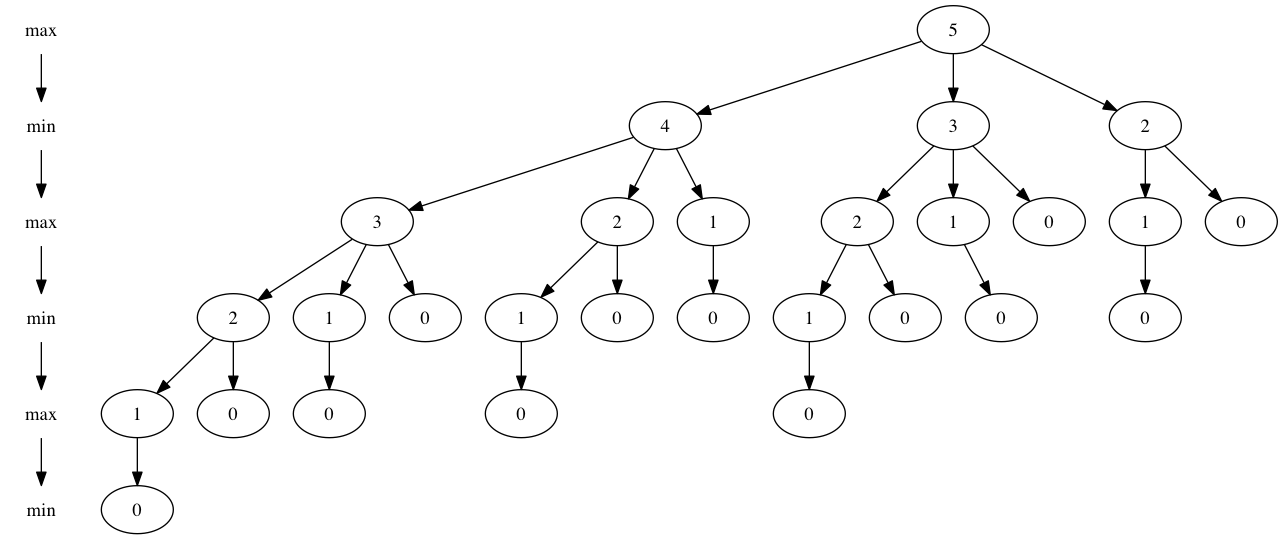
\includegraphics[scale=0.2]{images/5_minmax.png}\\
(a)\\
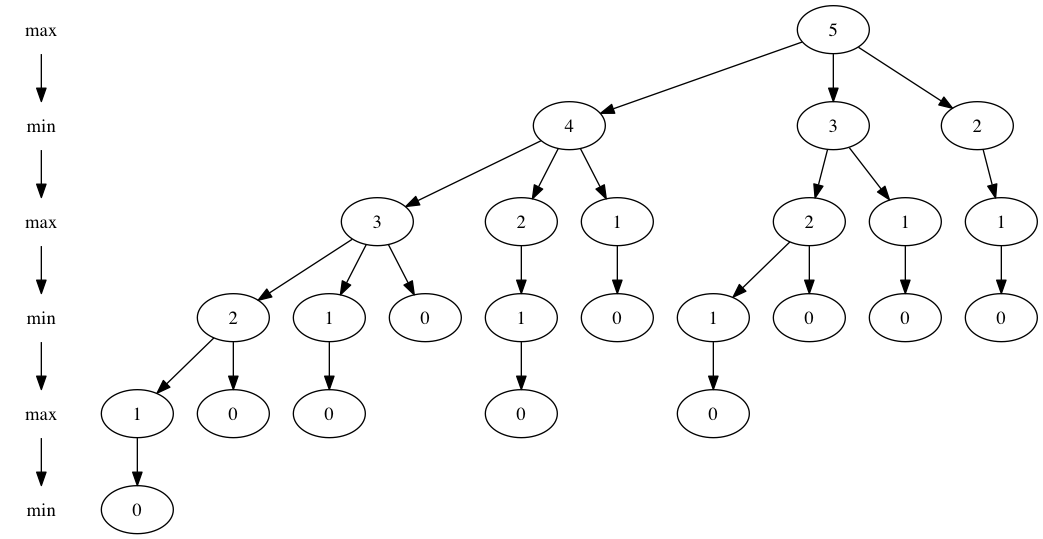
\includegraphics[scale=0.2]{images/5_ab.png}\\
(b)
\caption{Game tree of 5 matches: (a) using MinMax algorithm, 28 nodes; (b) using alpha-beta search algorithm, 25 nodes.}\label{fig:tree5}
\end{figure}

\section{Introduction}
In this project, two algorithms, MinMax search and Alpha-Beta search are implemented to play a simple match taking game.
The game starts with a pile of $n$ matches, where 2 players take turns to remove \textit{one}, \textit{two} or \textit{three} matches from the pile. The player who removes the last matches loses the game.

\section{Algorithm}
The state of the game, $s$, is defined as a tuple $(p, n)$ where $p$ is the player (Max or Min) and $n$ is the number of remaining matches. It is obvious that the terminal state of this game is the state with 0 match, i.e. $s.n = 0$. The utility for terminal state is defined as:
\[
f(s) = \left\{\begin{split}
& 0\text{~if~s.p=Min}\\
& 1\text{~if~s.p=Max}\\
\end{split}\right.
\]
The utility is chosen such that the first player always maximize utility and the other player always minimize it.
\subsection{Min-Max Algorithm}
The Min-Max search algorithm recursively search for optimal action at a given state: if the player is Max, it chooses the action that maximizes the utility returned from evaluating all possible moves; otherwise it chooses the action that minimizes the returned utility. At terminal states, the utility value is obtained with the definition in previous section.

\subsection{Alpha-Beta Search Algorithm}
Alpha-beta search is a variant of Min-Max search that prunes subtrees that do not affect decision making for current state. To do that, two values, i.e. alpha and beta, are record in the min-max search process to denote the best value ever found for player Max and Min. Any action that produces worse result the the best found result will not be investigated further, therefore reducing the total number of actions for evaluation. The experiments run in this project demonstrated the effectiveness of alpha-beta pruning.

\begin{figure}[htbp]
\center
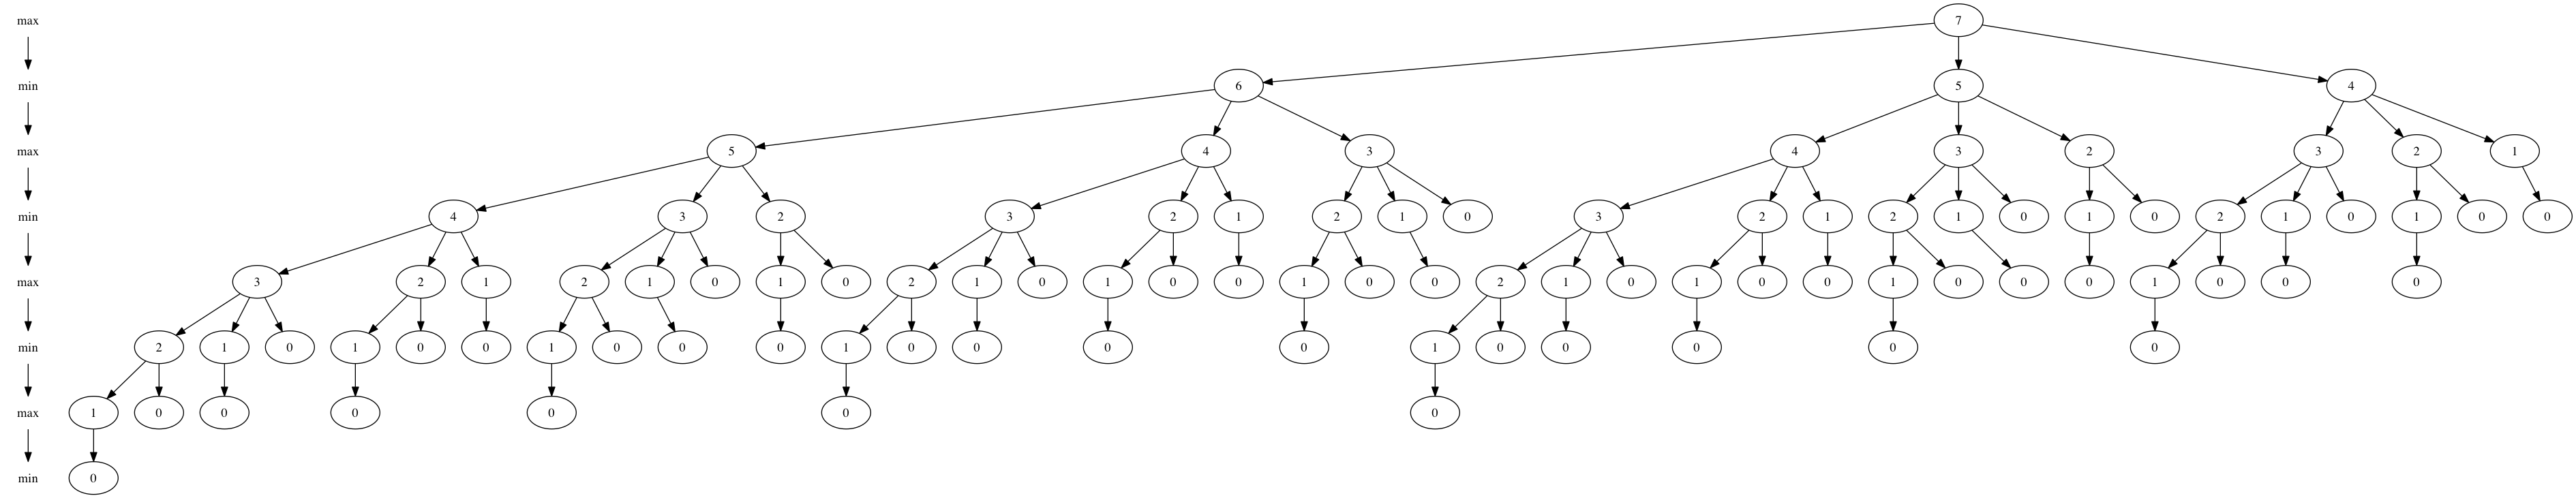
\includegraphics[scale=0.1]{images/7_minmax.png}\\
(a)\\
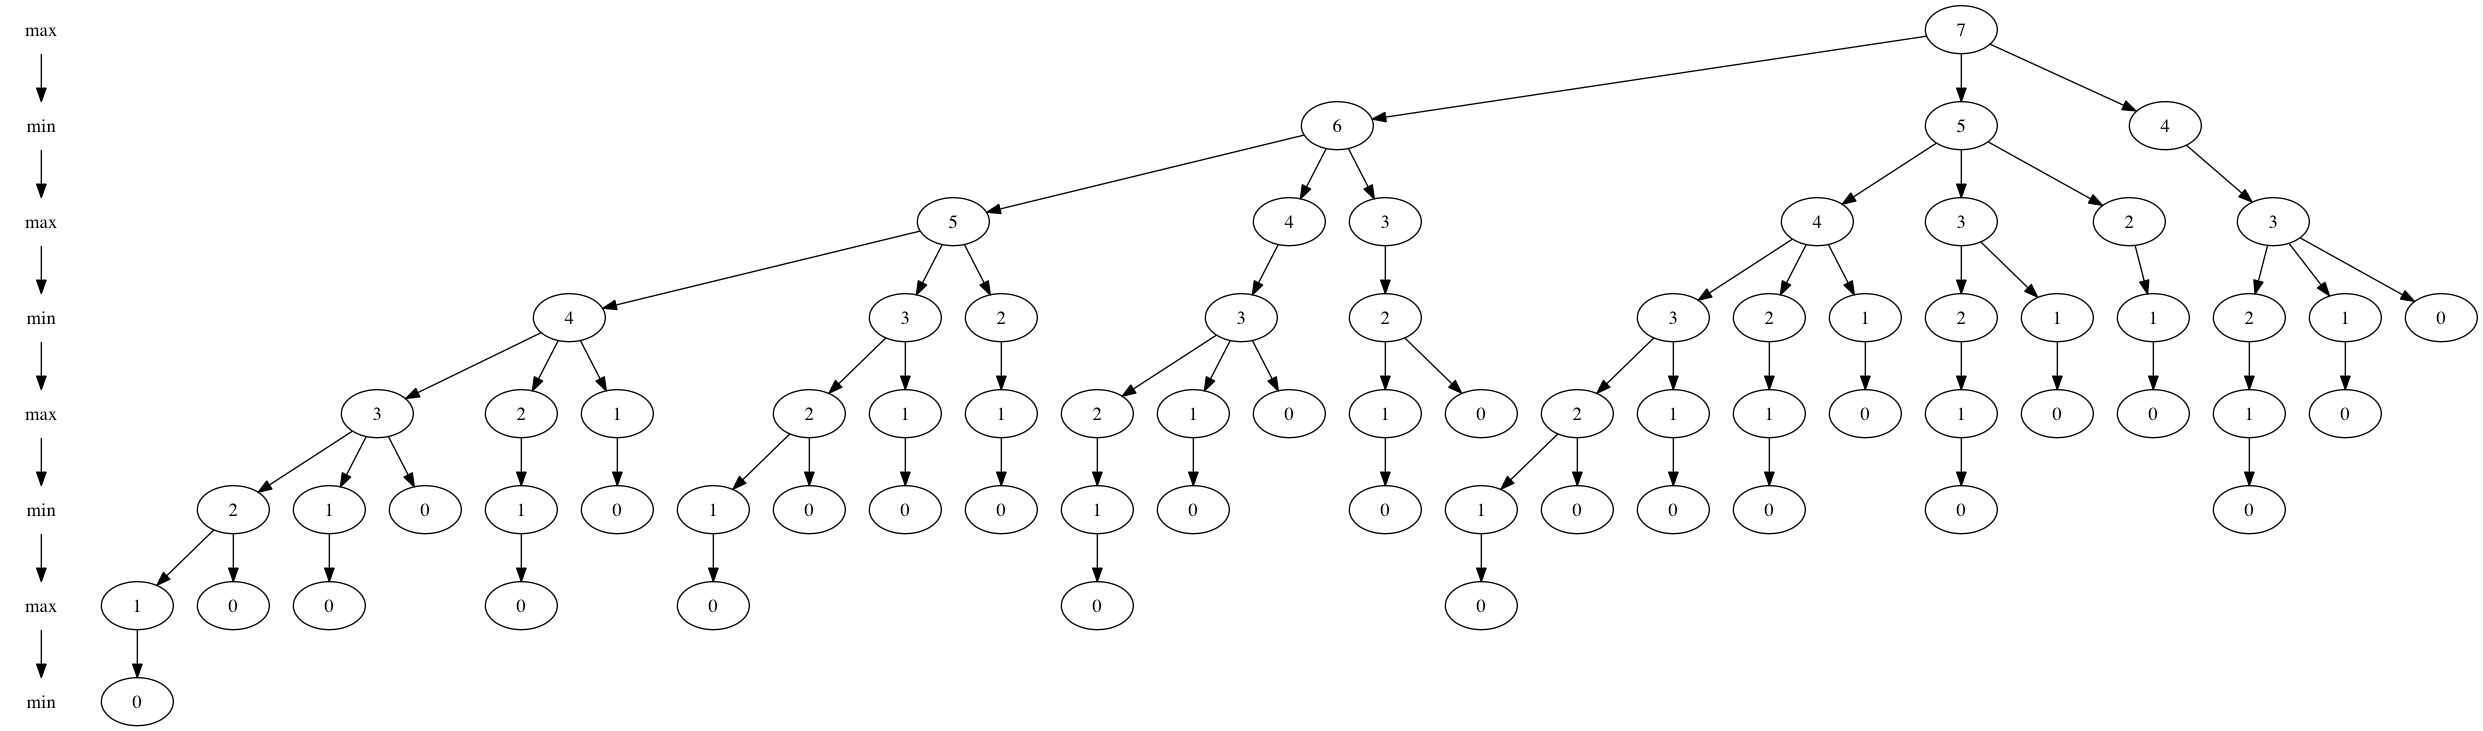
\includegraphics[scale=0.1]{images/7_ab.png}\\
(b)
\caption{Game tree of 7 matches: (a) using MinMax algorithm, 96 nodes; (b) using alpha-beta search algorithm, 71 nodes.}\label{fig:tree7}
\end{figure}

\section{Analysis}
\subsection{Comparison of Algorithms}
\begin{table}[htbp]
\center
\begin{tabular}{c|cc|c}
\hline
Number of Matches & MinMax & Alpha-Beta Search & Relative Size\\
\hline
5 & 28 & 25 & \pgfmathparse{25.0/28.0}\pgfmathresult\\
7 & 96 & 71 & \pgfmathparse{71.0/96.0}\pgfmathresult\\
15 & 12640 & 3241 & \pgfmathparse{3.241/12.640}\pgfmathresult\\
21 & 489396 & 66341 & \pgfmathparse{6.341/48.9396}\pgfmathresult\\
23 & 1655616 & 137302 & \pgfmathparse{1.37302/16.55616}\pgfmathresult\\
\hline
\end{tabular}
\caption{Comparison of game tree size by MinMax algorithm and Alpha-Beta search. The size of a game tree is defined as the total number of nodes in the tree.}\label{tab:perf}
\end{table}
A comparison of the performance of MinMax algorithm and Alpha-Beta algorithm is listed in Table.~\ref{tab:perf}. It is clear that the alpha-beta pruning produce much smaller game trees. For a game with 21 matches, the tree by alpha-beta algorithm is only about 13\% of the tree by min-max algorithm; the relative size of the alpha-beta game tree is even smaller than 10\% of that by min-max algorithm for a game with 23 matches.

Figure.~\ref{fig:tree5} and \ref{fig:tree7} shows the game trees generated by both algorithms for a game with 5 and 7 matches, respectively.
\subsection{Optimal Strategy and Moore Machine}
An interesting question about this game is whether opting to go first plays a role in the result of the game. It turns out the answer is yes, assuming both players are playing optimally. By running producing game trees for games with 5 to 21 matches, a pattern becomes clearly visible:
\begin{table}[htbp]
\center
\begin{tabular}{c|c||c|c||c|c||c|c}
\hline
$n$ & Who Wins & $n$ & Who Wins & $n$ & Who Wins & $n$ & Who Wins\\
\hline
5 & second & 9 & second & 13 & second & 17 & second\\
6 & first & 10 & first & 14 & first & 18 & first\\
7 & first & 11 & first & 15 & first & 19 & first\\
8 & first & 12 & first & 16 & first & 20 & first\\
\hline
\end{tabular}
\end{table}
Without doubt, for $n=1$ and $n=21$, the player goes second wins. That said, depending on the initial number of matches, going first or second will lead to opposite outcome in an ideal game.

In case of an optimal player against a random player, the optimal player can always win. The reason is the optimal player could choose to go first or second based on the initial number of matches, and for each initial state, the outcome of the game can be completely determined by one player. 

To see the reason why the assertion above is true, let's consider the optimal strategy of the game first.

From Table.~\ref{tab:perf} we may conjecture that the second player can always win if the initial state has $n = (4k+1)$ matches, otherwise the first player can always win. This is in fact true.

Consider the initial state with only 1 match, the first player is guaranteed to lose, so the second player must win.

For initial state with 2, 3, 4 matches, the first player can always force the second player to remove the last match by removing 1, 2, or 3 matches. Therefore, the first player is guaranteed to win in these cases.

Consider the initial state with 5 match, the first player is again guaranteed to lose. This is because no matter how many matches the first player removes, the second player can always remove just enough matches to leave only 1 match in the pile. Suppose the first player removes $m$ matches, the second player can to remove $4-m$ matches. In total, they always remove 4 matches in the first two rounds, leaving the last match for the first player to remove.

This is also true for initial states with $4k+1$ matches (5, 9, 13, 17, 21, ...), when the second player can always win by using the strategy describe above. 

For initial state with $4k + l$ matches ($l=0, 2, 3$), the first player is therefore guaranteed to win by removing $[(l-1)\mod 4]$ matches in the first round, leaving $4(k-1)+1$ matches in the pile. This sets the second player in the case with $4k+1$ matches initial state, in which the player go first would always lose. To win the game, the first player only needs to remove $4-x$ matches in later rounds, following the strategy mentioned above, where $x$ is the number of matches the second player removes.

To sum up, the optimal strategy for playing this game can be described with the Moore machine below:

\begin{center}
\digraph[scale=0.4] {Moore} {
    node [shape=circle];
	1->1 [label="x=3"];
	1->2 [label="x=2"];
	1->3 [label="x=1"];
	2->1 [label="x=3"];
	2->2 [label="x=2"];
	2->3 [label="x=1"];
	3->1 [label="x=3"];
	3->2 [label="x=2"];
	3->3 [label="x=1"];
	s->1 [ label="n=4k+2" ];
	s->2 [ label="n=4k+3" ];
	s->3 [ label="n=4k" ];
	s->s [ label="n=4k+1"];
	s [shape=doublecircle];
	{rank=same; s}
	{rank=same; 1}
	{rank=same; 3}
	{rank=same; 2}
}
\end{center}
The labels on the edge represents the opponent's move, and the node $s$ represents the initial state. The number in each node represents the number of matches to remove for current action, i.e. the output of the Moore machine. For example, if the current state is node 1, the next state is still node 1 if the opponent removes 3 matches; if the opponent removes 2 matches, the next state is node 2 (i.e. remove 2 matches); otherwise the next state is node 3. The looping edge of node $s$ represents that in case of $n=4k+1$, let the opponents move first and make decision by treating the resulting pile as initial state.
\end{document}